\documentclass{article}

\usepackage[english]{babel}
\usepackage{svg}
\usepackage{titling}

% Set page size and margins
% Replace `letterpaper' with `a4paper' for UK/EU standard size
\usepackage[letterpaper,top=2cm,bottom=2cm,left=3cm,right=3cm,marginparwidth=1.75cm]{geometry}

% Useful packages
\usepackage{amsmath}
\usepackage{graphicx}
\usepackage[colorlinks=true, allcolors=blue]{hyperref}

\usepackage[T1]{fontenc}
\usepackage{beramono}
\usepackage{listings}
\usepackage{xcolor}
\usepackage{float}

\definecolor{dkgreen}{rgb}{0,0.6,0}
\definecolor{gray}{rgb}{0.5,0.5,0.5}
\definecolor{mauve}{rgb}{0.58,0,0.82}

% Context, modifications, background (how it was before)
% Why is it a problem?
% Contributions (my beautiful story)



\lstdefinestyle{sc}{
  frame=tb,
  language=scala,
  aboveskip=3mm,
  belowskip=3mm,
  showstringspaces=false,
  columns=flexible,
  basicstyle={\small\ttfamily},
  numbers=none,
  numberstyle=\tiny\color{gray},
  keywordstyle=\color{blue},
  commentstyle=\color{dkgreen},
  stringstyle=\color{mauve},
  frame=single,
  breaklines=true,
  breakatwhitespace=true,
  tabsize=3,
}

\lstset{style=sc}


\title{Bachelor project\\Adding support for Scala-CLI on Scastie}
\date{Summer 2023}
\author{Marwan Azuz, \href{mailto:marwan.azuz@epfl.ch}{marwan.azuz@epfl.ch}
\\ Supervised by Julien Richard-Foy (Scala Center) and Jędrzej Rochala (VirtusLab)}

\begin{document}

\begin{titlingpage}
\maketitle
\begin{figure}[ht]
    
\includegraphics[width=.4\linewidth]{logos/scala-center-logo-black@2x.png}
    \hfill
    
\includegraphics[width=.4\linewidth]{logos/epfl.png}
\end{figure}
\end{titlingpage}

\newpage


This document contains a lot of clickable links, that can be used to jump on specific code or documentation.
Feel free to read it on a PDF viewer instead of printing it. You are saving some trees!


\tableofcontents

\section{Introduction}


\subsection{Presentation of Scastie}

Scastie is an interactive playground for Scala in the browser, available at \href{https://scastie.scala-lang.org/}{scastie.scala-lang.org}.
It offers a quick and easy way to write Scala code in an interactive manner, similar to worksheets.

\begin{figure}[H]
    \centering
    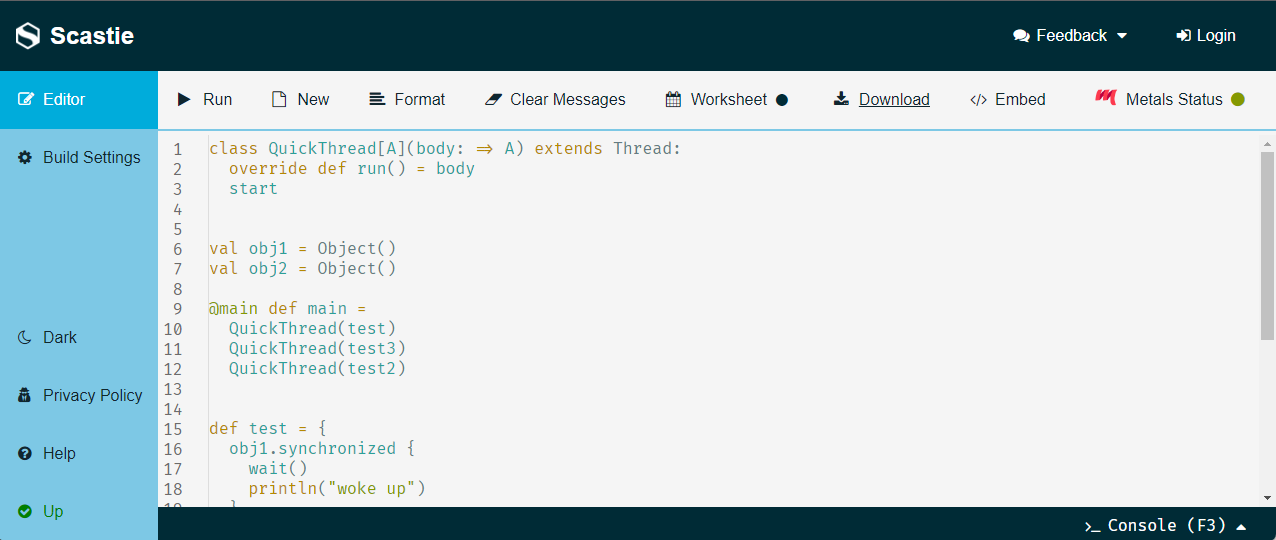
\includegraphics[width=0.7\columnwidth]{scastie_main.png}
    
    \caption{Using Scastie to run code for demonstration purposes on the CS-206 Parallelism \& Concurrency course at EPFL.}
\end{figure}

In the same manner as worksheets, it offers a preview of intermediate values~:

\begin{figure}[H]
    \centering
    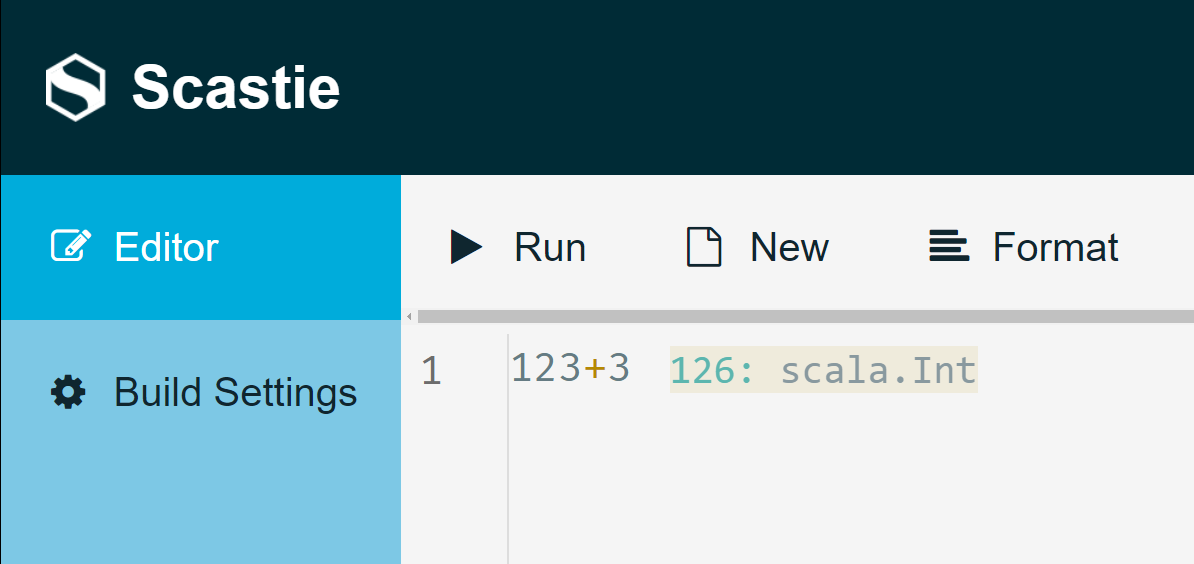
\includegraphics[width=0.7\columnwidth]{scastie_instrumentation.png}
\end{figure}

and also features autocompletions using Metals~:

\begin{figure}[H]
    \centering
    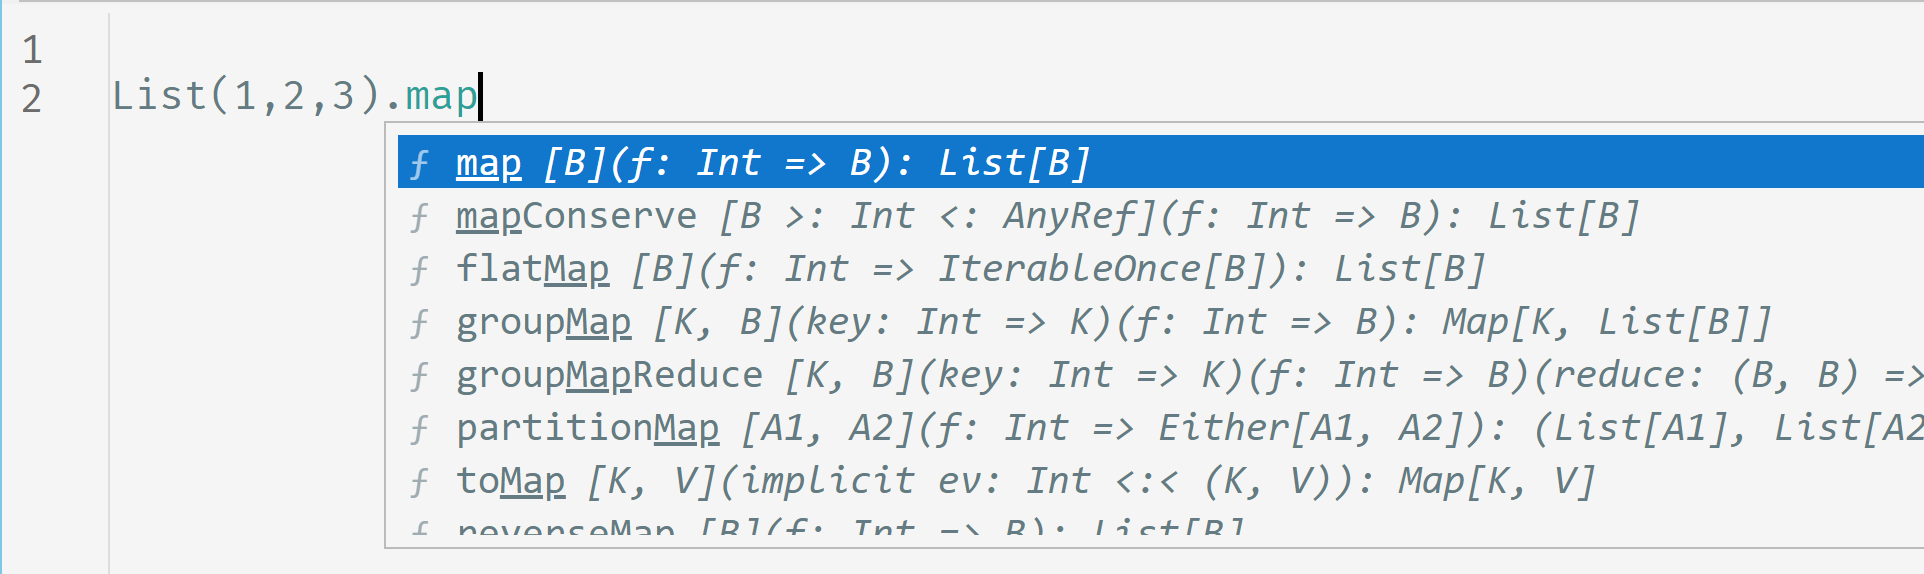
\includegraphics[width=0.7\columnwidth]{scastie_autocomplete.png}
\end{figure}

\subsection{Usage of Scastie~?}

Scastie is great to have a worksheet right in the browser, accessible from any device.
When teaching the Scala language, it can be a quite handy tool as the following tweet demonstrates~:

\begin{figure}[h!]
    \centering
    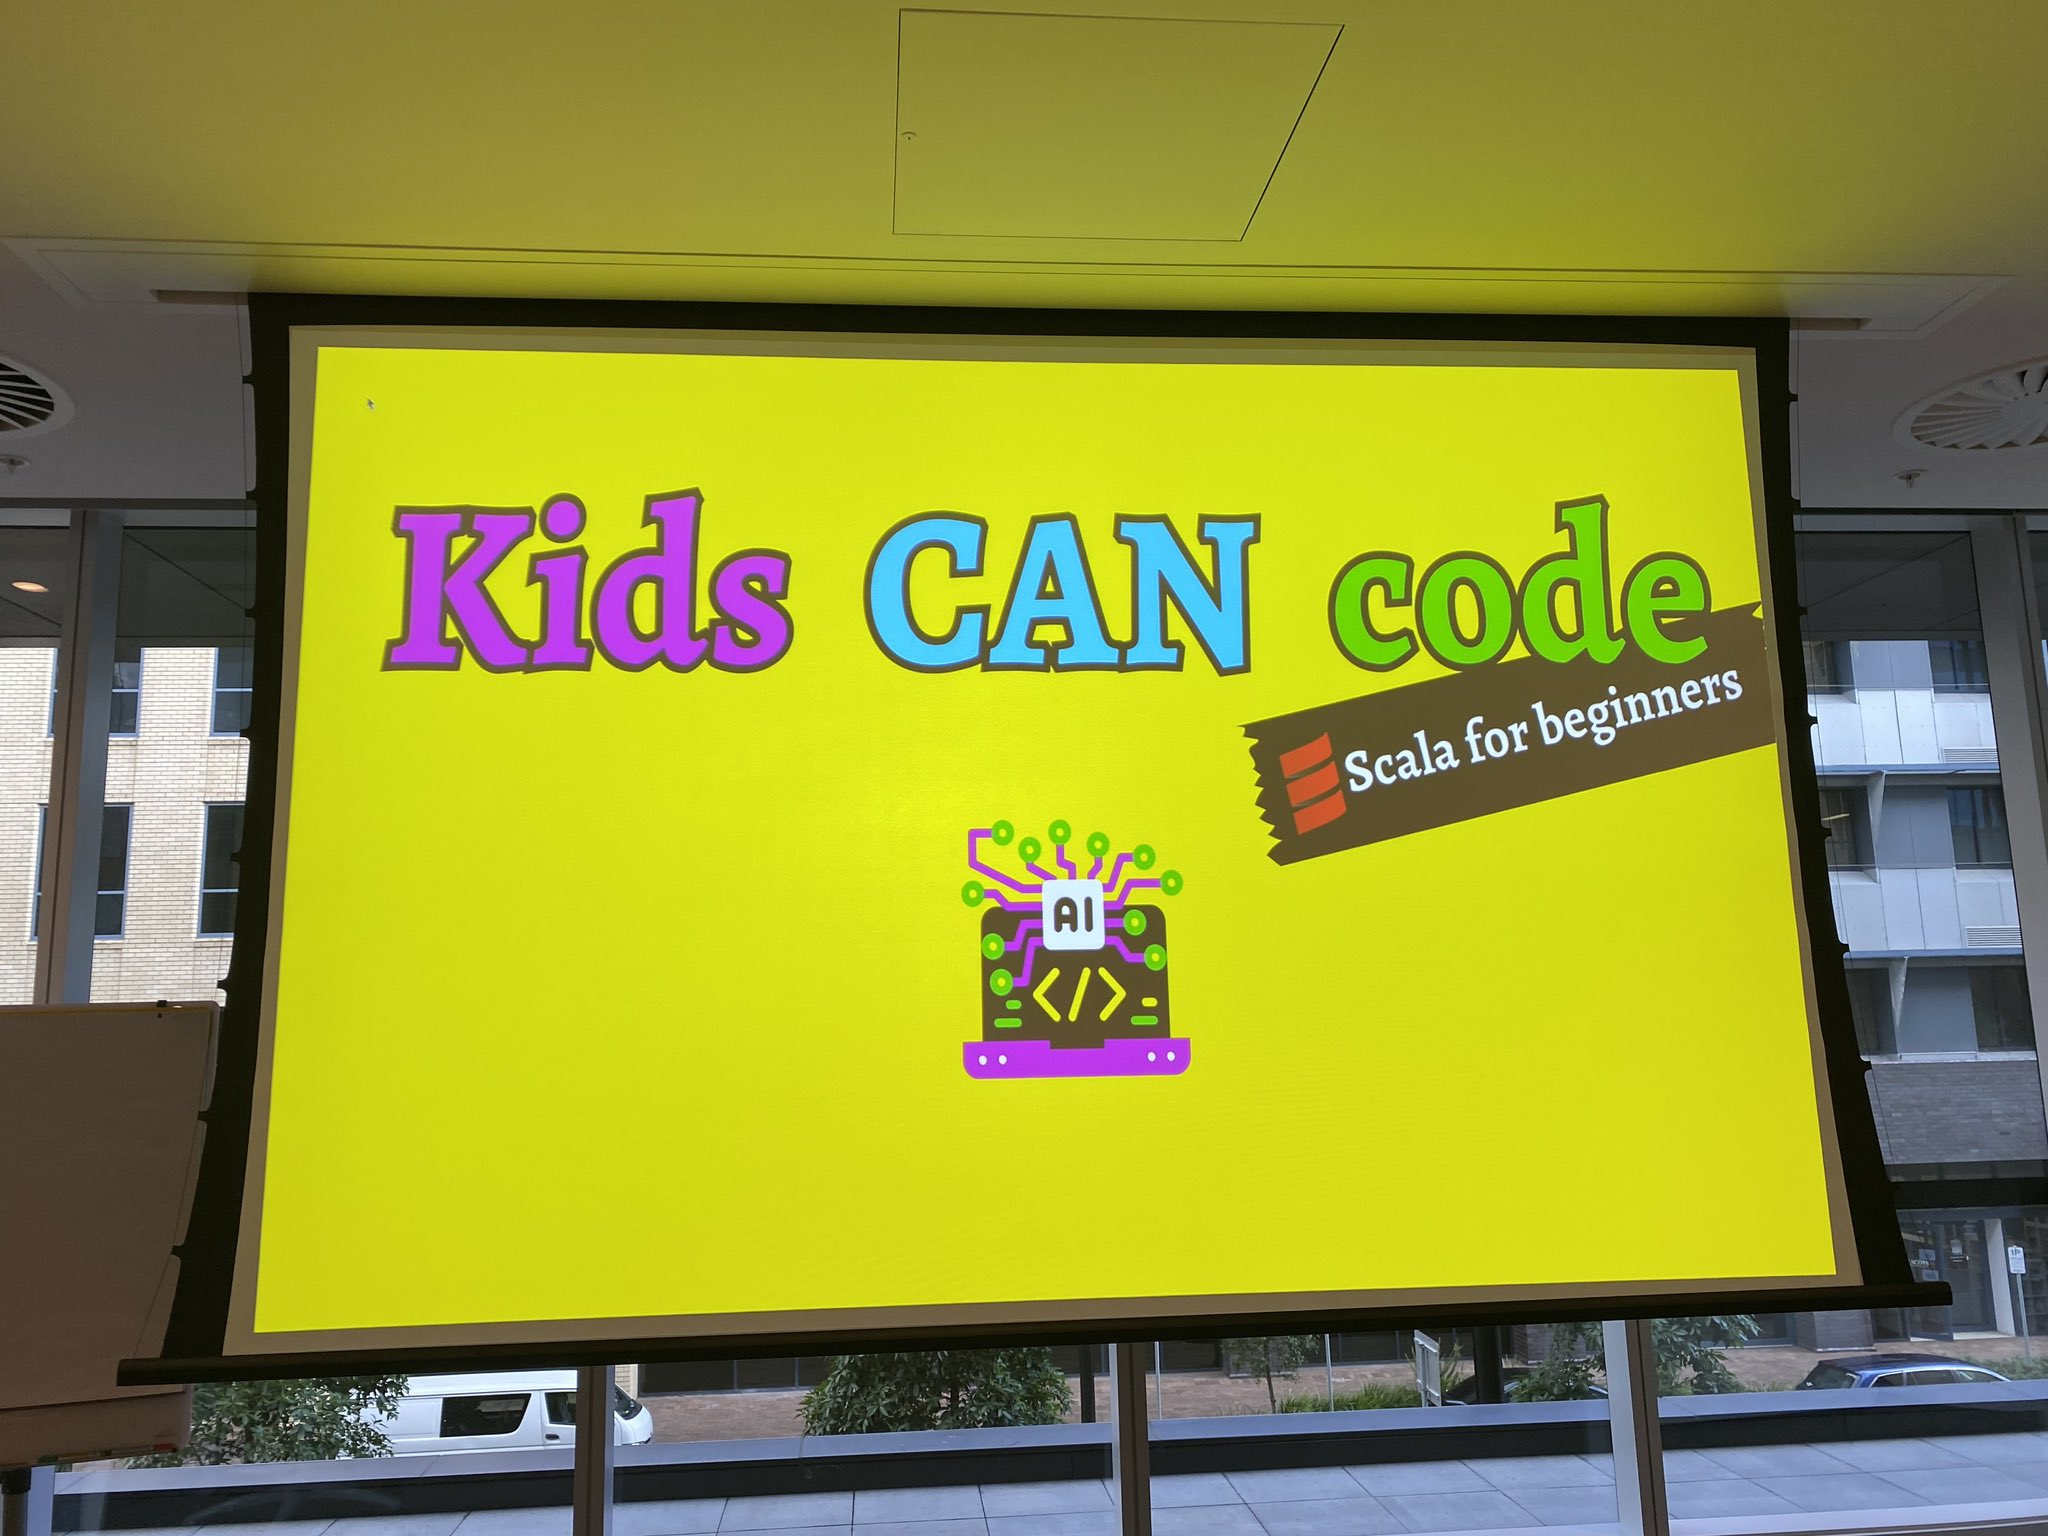
\includegraphics[width=.3\linewidth]{tweet/1.jpg}
    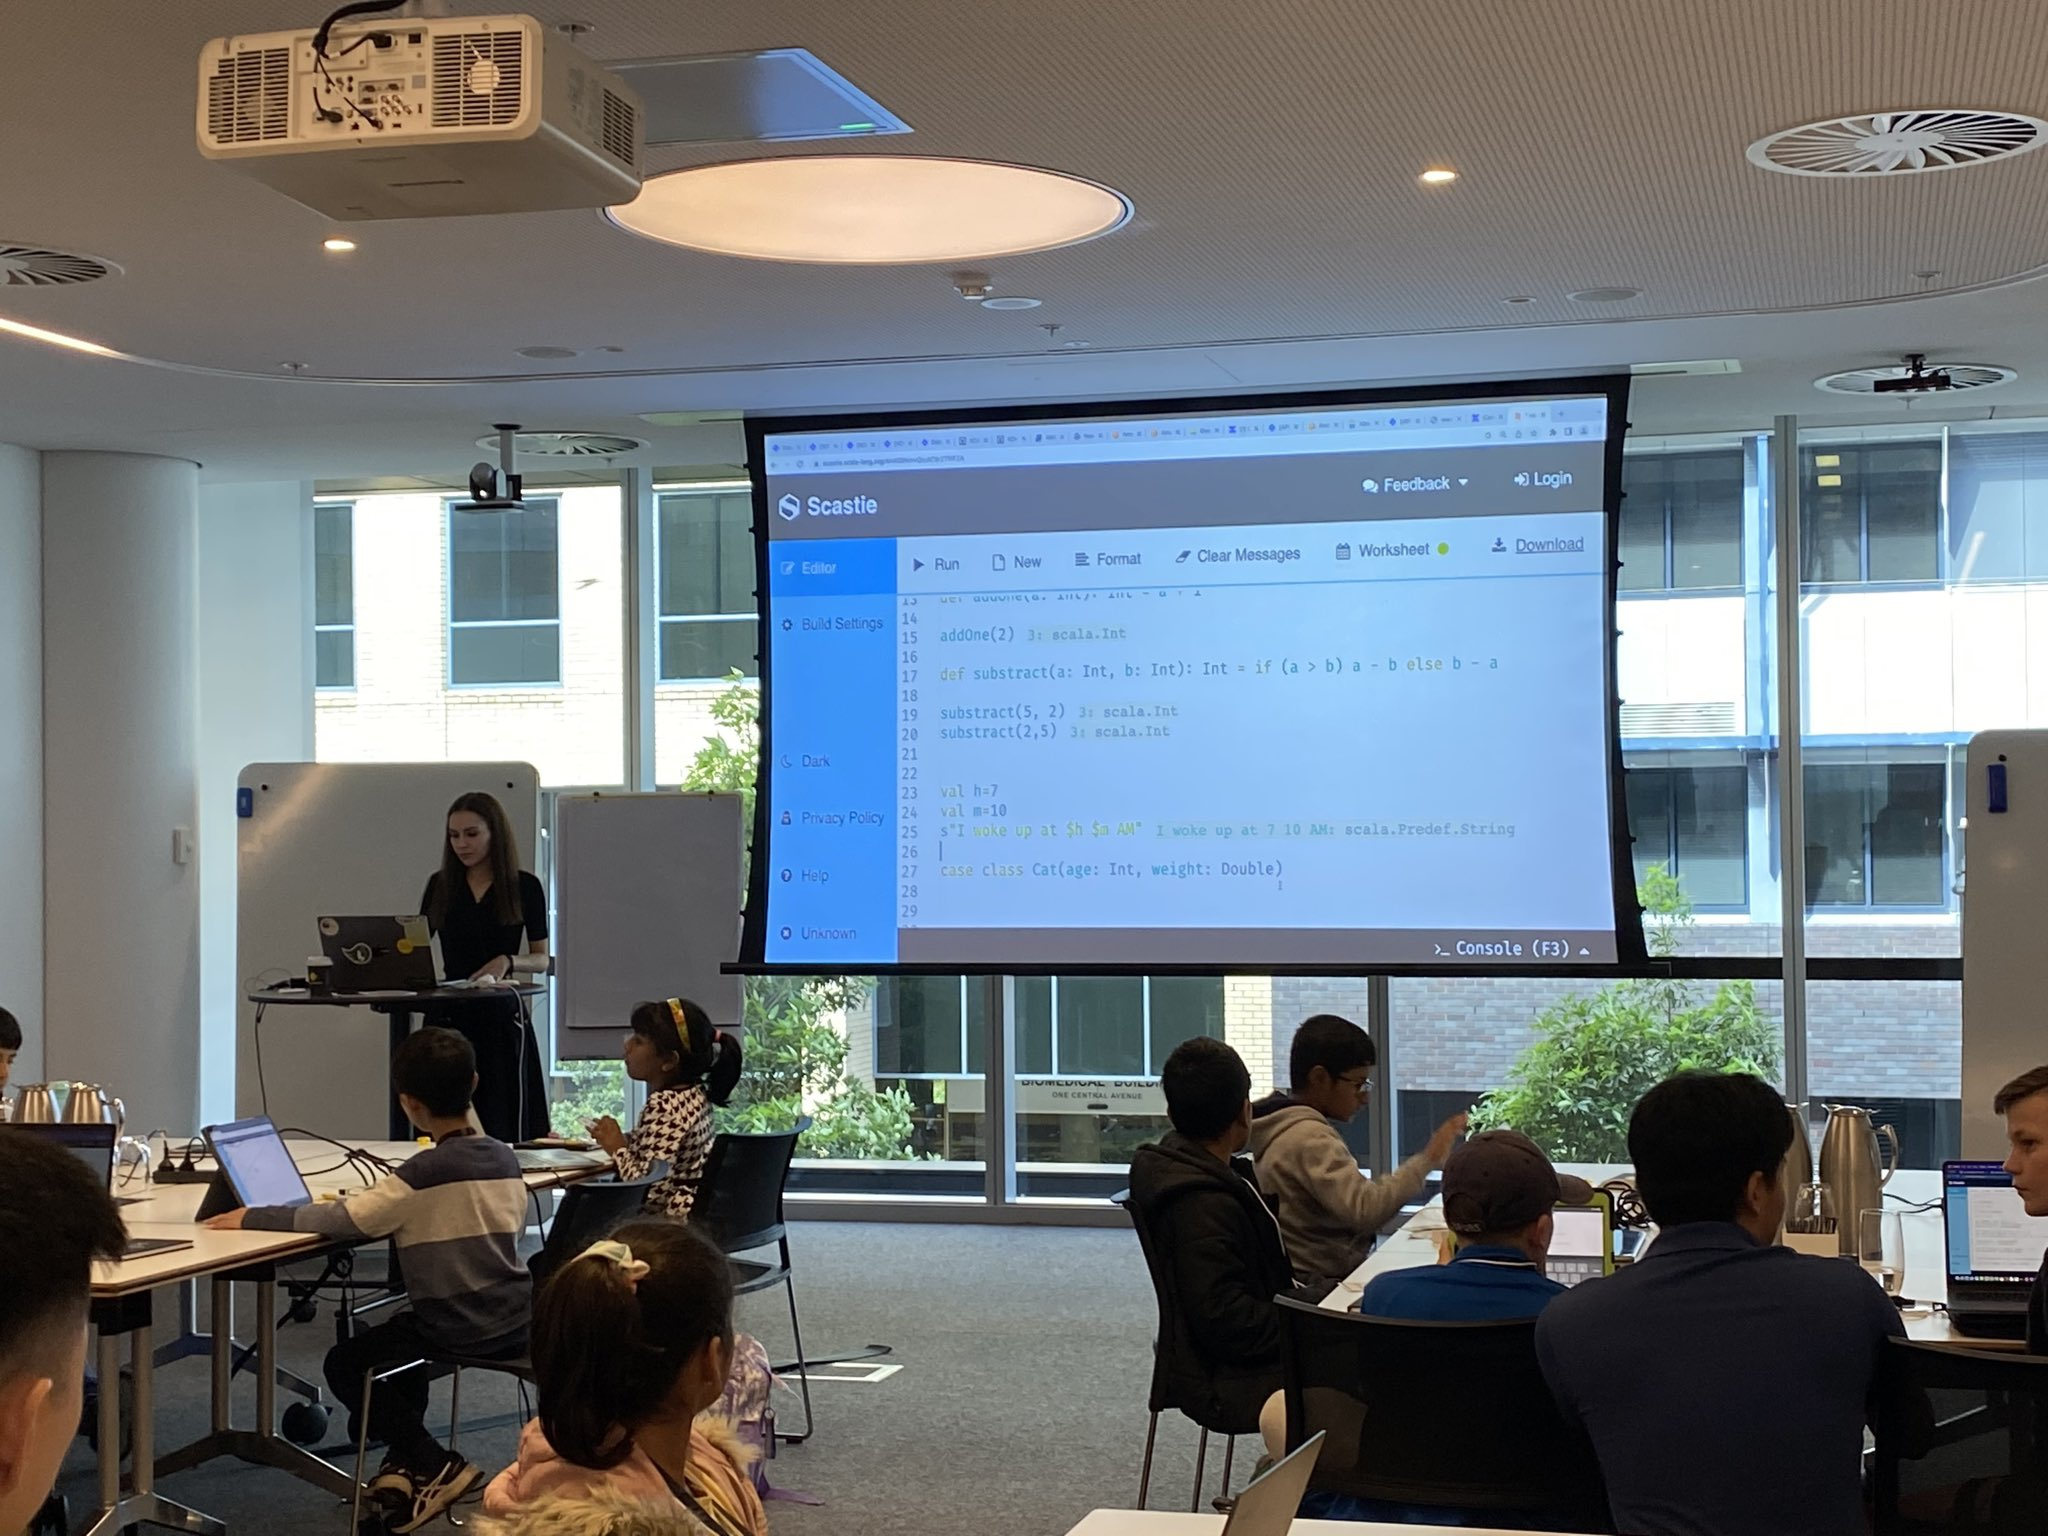
\includegraphics[width=.3\linewidth]{tweet/2.jpg} \\
    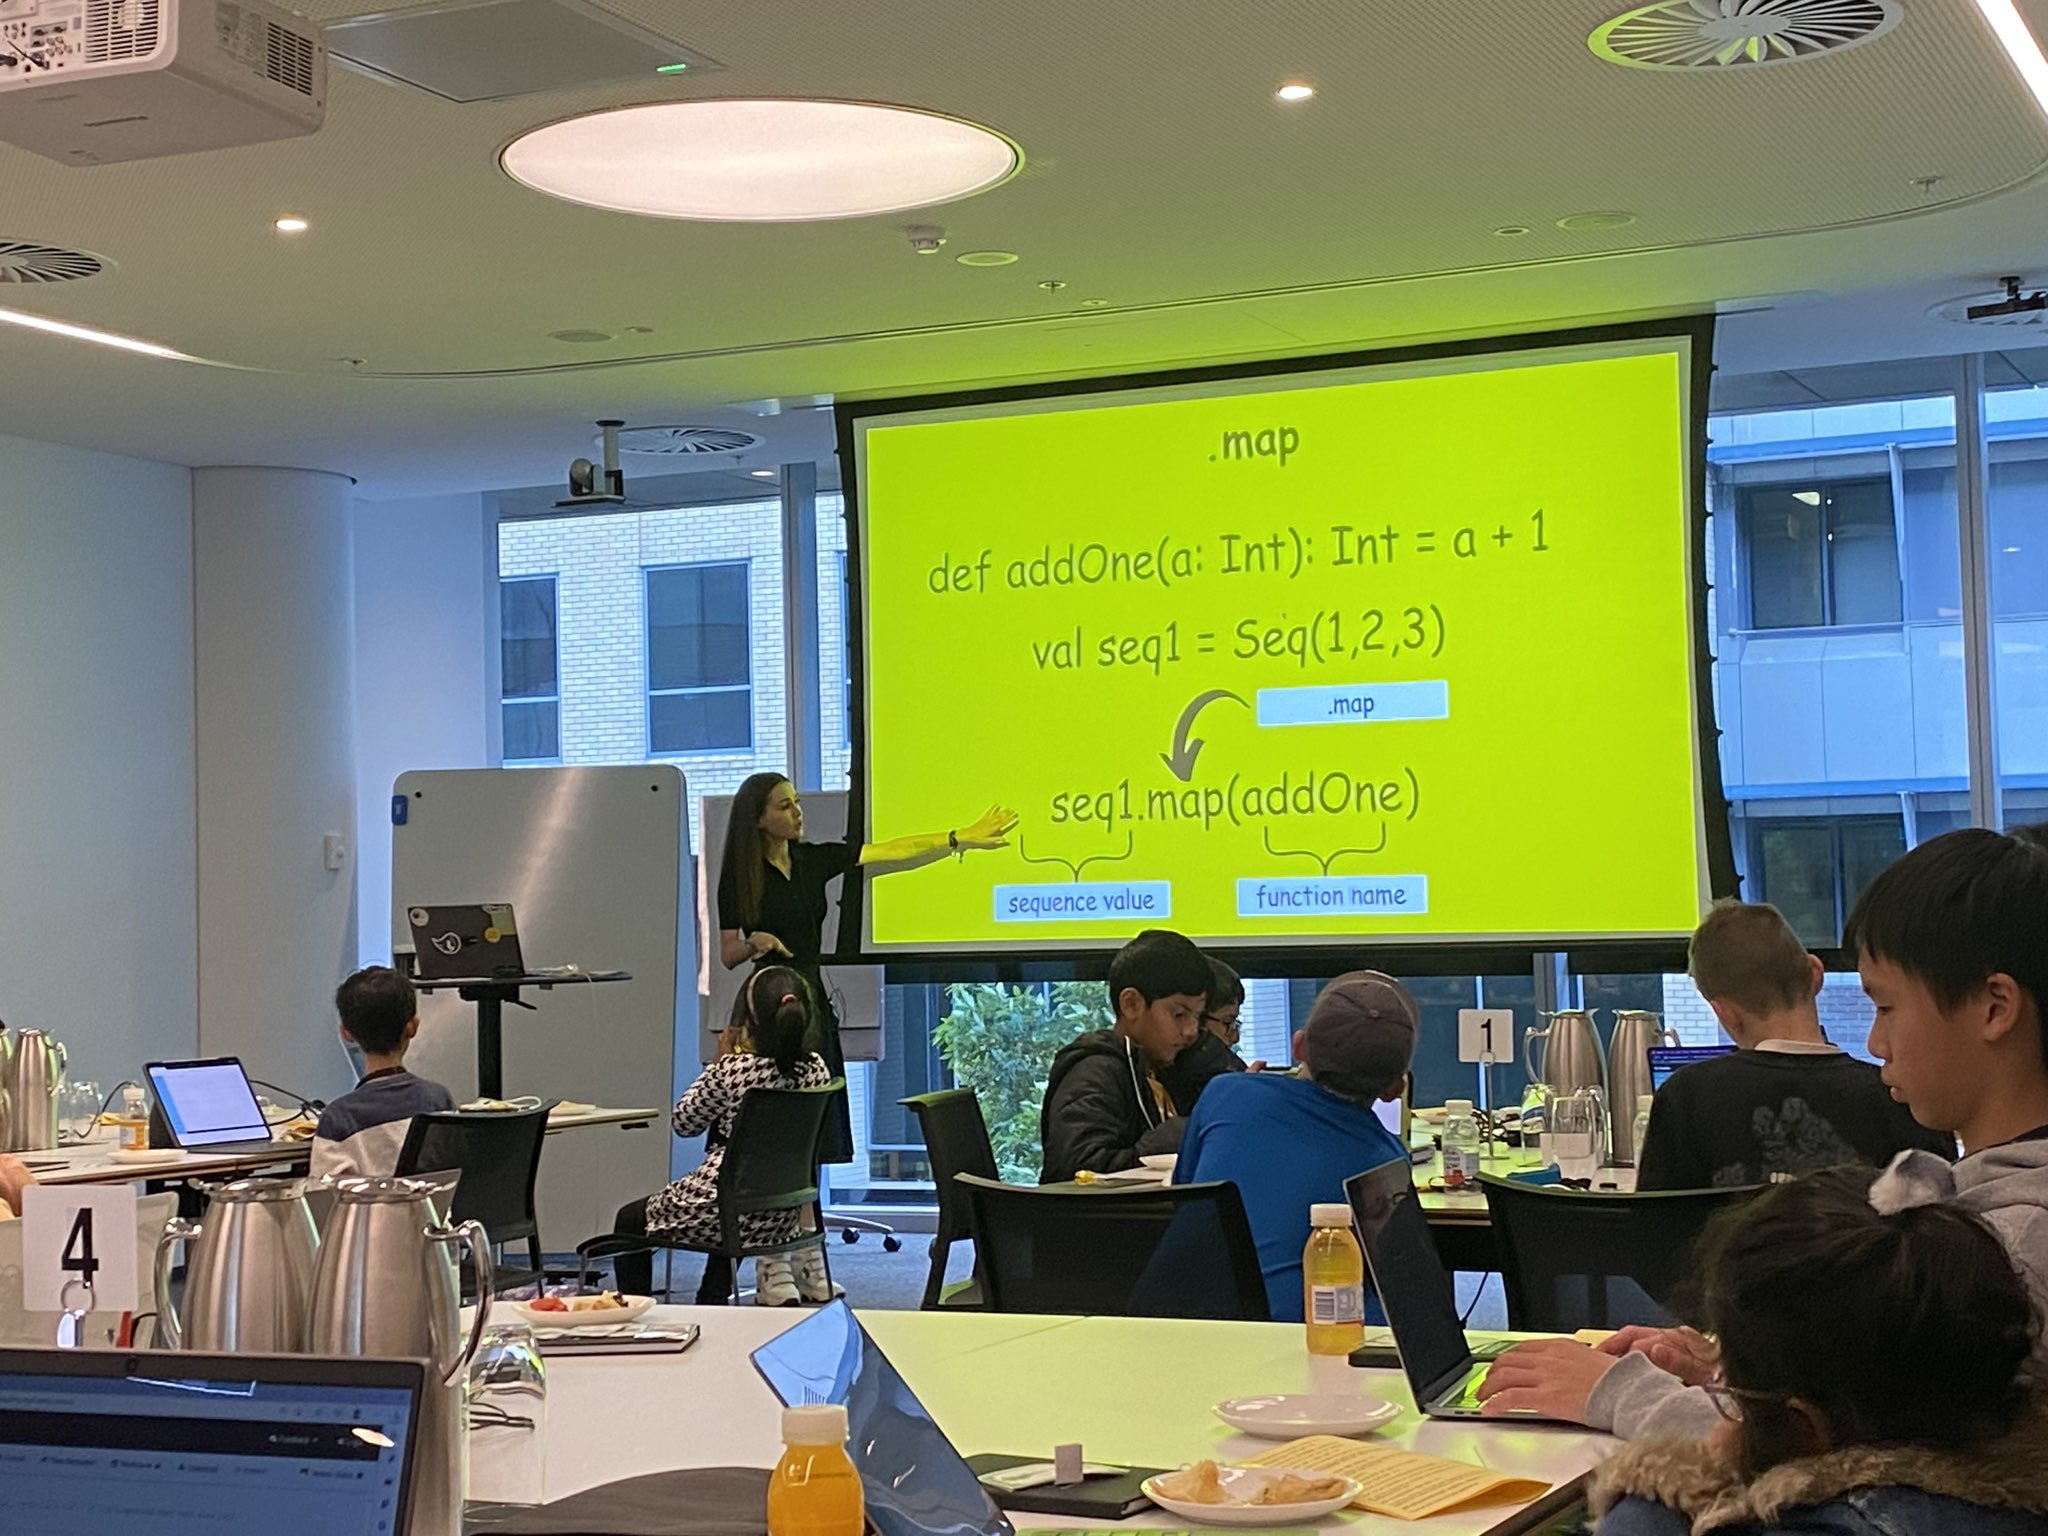
\includegraphics[width=.3\linewidth]{tweet/3.jpg}
    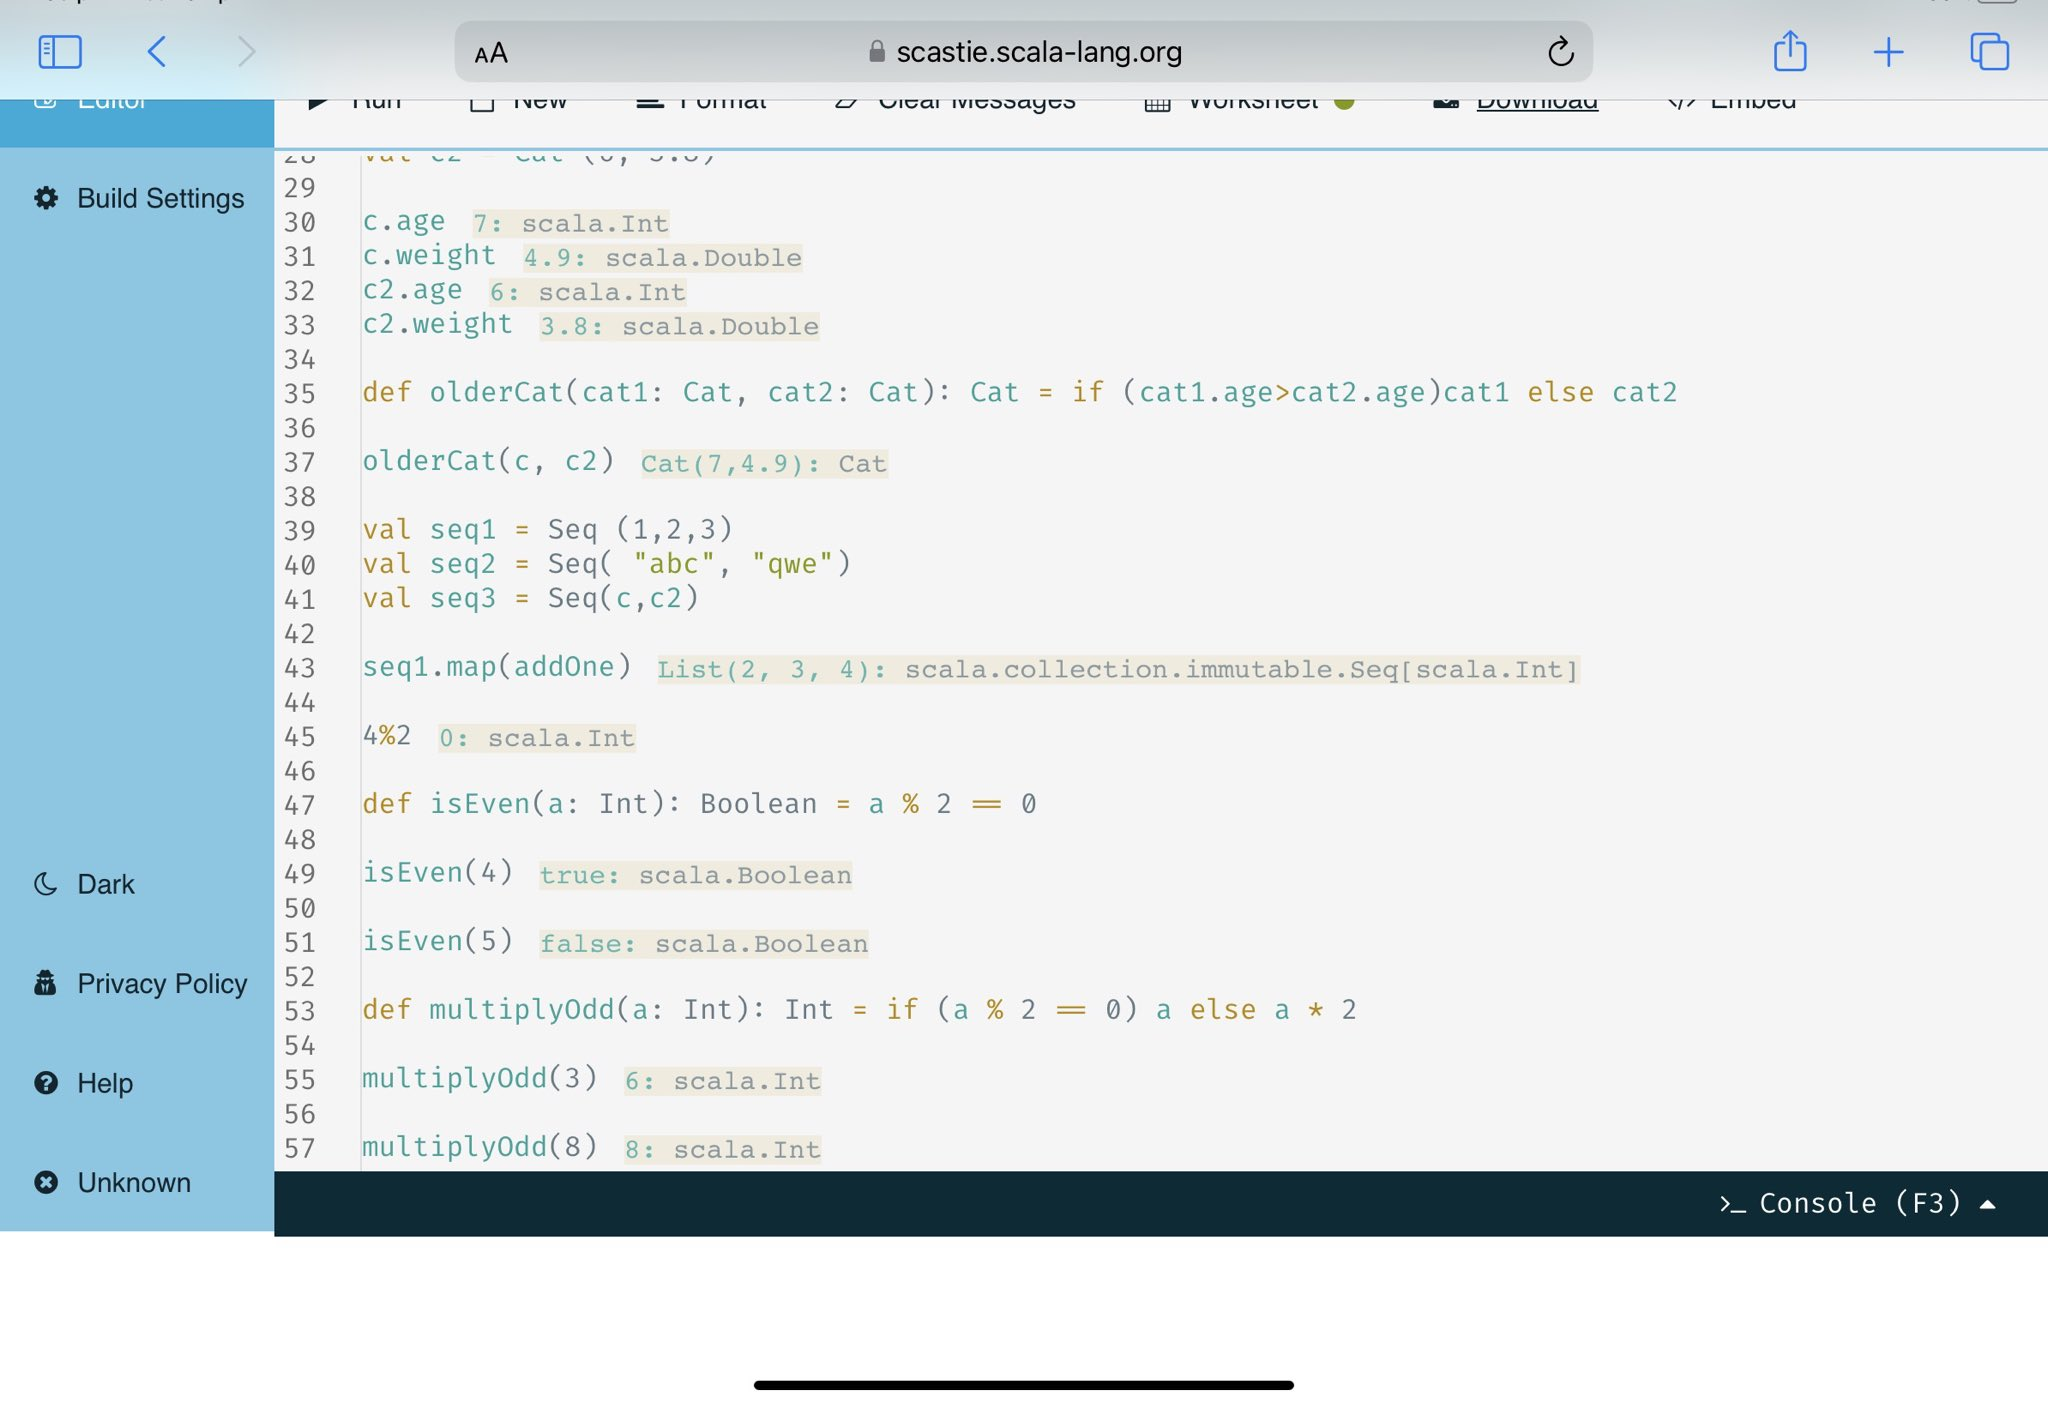
\includegraphics[width=.3\linewidth]{tweet/4.jpg}
    \caption{Tweet from \href{https://twitter.com/BesseIFunction/status/1648560454975868933}{@BessieIFunction} learning kids Scala using Scastie}
\end{figure}

It supports adding libraries in a user-friendly interface and also sharing snippets in a hassle-free way~:
perfect to demo the usage of a library or Scala feature~!

\subsection{The issue with Scastie}

Scastie has a little flaw in how it runs snippets~: when using a configuration that is not the default configuration
(i.e. specific Scala version and/or libraries), it can have a lot of delay when running a snippet.
To explain more in detail this problem, let's go with a quick overview of how Scastie works.
Scastie is a distributed system and has different components. Here a quick visual representation of the architecture~:

\begin{figure}[h!]
    \centering
    \includesvg[width=0.9\columnwidth]{architecture.svg}
    \label{fig:scastie_architecture}
    \caption{Quick visual overview of Scastie's architecture}
\end{figure}

When an user submits a snippet to be ran, it passes through the dispatcher that sends it to the load balancer that forwards it to one of the
available runners.

One of the current issues with Scastie is how it handles libraries and is linked with how SBT handles it.
On a local SBT project, one should add the library in the configuration file \lstinline{build.sbt} and then reload SBT.
Keep in mind that reloading SBT is an operation that takes a lot of time and makes the specific runner busy.
If one user wants to use -- for instance \lstinline{com.lihaoyi::os-lib} --, the load balancer will try to find a runner that has
the library already loaded.

More generally, one can define 'configuration': the set containing the Scala version and libraries. The load balancer will try to find a
runner that has the same configuration as the required one to run a specific snippet -- to avoid reloading unnecessarily a runner.
If it manages to find such a runner, it forwards the execution. Otherwise, it will ask for a runner to reload with the
required configuration. This creates a lot of overhead -- hence, a lot of latency to the user -- to execute a snippet.

The goal of this project is to replace SBT by Scala-CLI~: a faster Scala runner. We can safely assume that the utterly complex Scala Build
Tool represents a too much convoluted tool to be used on Scastie, which main role is to execute quick user snippets.
Therefore, Scala-CLI seems to be a suitable replacement for SBT.

\subsection{Scala-CLI directives}

Adding Scala-CLI offers for a quick and easy way to specify how Scala should be ran. The two most important ones are~:

\begin{lstlisting}[style=sc]
//> using scala "2"

object HelloWorld extends App {
    println("Hello world!")
}
\end{lstlisting}

which defines the Scala version (here, the latest Scala 2 version.) and

\begin{lstlisting}[style=sc]
//> using dep "com.lihaoyi::os-lib:0.9.1"

@main def main = println("Hello world")
\end{lstlisting}

which adds the dependency \lstinline{com.lihaoyi::os-lib:0.9.1}.

Let's note that Scastie must support those directives (including Metals and the Scala-CLI runner.)

\subsection{Timeline of the project}

The project has been decomposed into the following milestones~:

\begin{enumerate}
    \item The project works on the student's computer.
    \item The Scala-CLI runner can execute Scala code.
    \item The runner is correctly implemented.
    \item Metals is working correctly along with dependencies.
    \item The runner is connected to the website with the UI to support it.
\end{enumerate}

The report will follow an almost linear approach of all the milestones achieved during this project,
that has been done in the context of a mandatory semester project at EPFL.

\section{The birth of the Scala-CLI runner}

Multiple solutions about how to interact with Scala-CLI have been thought. Here is a list with explanations on every of these approach.

From now on, we will refer to "script" as a general Scala file: it could be a worksheet or a standalone Scala file.

\subsection{The most basic runner -- ever}

A first way of tackling this problem would be to let Scala-CLI in charge of everything: compiling and running the script. Not even bothering to save the script to a file: pipe the script to the standard input of Scala-CLI and get the result of it. This enables for a single runner to execute multiple scripts at the same time.

\begin{figure}[h!]
    \centering
    \includesvg[width=0.9\columnwidth]{scli_1.svg}
    \caption{The most basic runner}
\end{figure}

Spawning a process, piping content to the input and listening the output can be easily done in Scala using the \href{https://dotty.epfl.ch/api/scala/sys/process.html}{scala.sys.process} package. Such a prototype can be found on commit \href{https://github.com/Maeeen/scastie/blob/a74627d080f70f664931133632f06f514a2856f8/scli-runner/src/main/scala/com.olegych.scastie.sclirunner/ScliActor.scala}{\lstinline{a74627d}, file \lstinline{ScliActor.scala}}

This solution is easy and quick. However, it is not resilient to compilation errors without extensive effort~: since the output is made to be shown in a terminal for a human, managing through such a solution requires proper parsing (which will be very likely unnecessarily complicated and archaic).

Here is an example~: 

\begin{lstlisting}[language=bash,frame=tb,basicstyle={\small\ttfamily},frame=single]
maeeen@Marwan-PC:~/test$ cat test.scala
@main def main = unknownfunction("hello")

maeeen@Marwan-PC:~/test$ scala-cli - < test.scala
Starting compilation server
Compiling project (Scala 3.2.2, JVM)
[error] stdin:1:30
[error] Not found: unknownfunction
Error compiling project (Scala 3.2.2, JVM)
Compilation failed
\end{lstlisting}

This is how Scastie handles SBT by default and it would be preferable to go with a more reliable option that offers interaction in a machine-understandable format.

A side remark~: my fellow student colleague working on Scastie implements multiple files support. Choosing such a solution and stopping here would require extra modifications to the runner to add such a feature.

\subsection{The Build Server Protocol at the rescue}

Many builds tools offer a protocol to interact with them. One of these protocols is the BSP (short for Build Server Protocol, see the specification on \href{https://build-server-protocol.github.io/docs/specification}{build-server-protocol.github.io/docs/specification}). Scala-CLI does offer a BSP server with the command line argument \lstinline{bsp}.

Interacting with the build server protocol is still done with the input and output streams of the child process, but using JSON with an extra-header. There exists multiple solutions to handle the BSP protocol but the most straightforward way is to use the \href{https://mvnrepository.com/artifact/ch.epfl.scala/bsp4j}{ch.epfl.scala::bsp4j} package on Maven. A similar artefact exists for Scala (\lstinline{ch.epfl.scala::bsp4s})~: however, it has not been updated after 2021 according to the Scaladex and had almost no documentation on its usage on the Build Server Protocol specification (by the time writing this report.)

\begin{figure}[h!]
    \centering
    \includesvg[width=0.9\columnwidth]{sclirunner.svg}
    \caption{Architecture of the Scala-CLI runner}
\end{figure}

In this configuration, the runner spawns a Scala-CLI server in BSP mode inside a temporary folder. Afterwards, the BSP client initializes the workspace to make it ready for executions.

Then, on every script that needs to be ran, the content of the user script is written to a \lstinline{main.scala} file, at the root of the project. Afterwards, the BSP client does the following tasks~:

\begin{enumerate}
    \item Reloading the workspace \href{https://build-server-protocol.github.io/docs/specification#reload-request}{\lstinline{workspace/reload}}~: to be sure that any dependencies changes is taken into consideration.
    \item Get build targets' id \href{https://build-server-protocol.github.io/docs/specification#workspace-build-targets-request}{\lstinline{workspace/buildTargets}}~: since Scala-CLI setups a new workspace, it has a specific build id. This id has to be specified for every request afterwards. Let's note that we take the first build target which is not a test build target.
    \item Compilation \href{https://build-server-protocol.github.io/docs/specification#compile-request}{\lstinline{buildTarget/compile}}~: Triggers the compilation of the workspace.
\end{enumerate}

\subsubsection{Running snippets: let Scala-CLI run the snippet}

\begin{enumerate}
    \setcounter{enumi}{3}
    \item Run \href{https://build-server-protocol.github.io/docs/specification#compile-request}{\lstinline{buildTarget/run}}~: let Scala-CLI runs by itself the script
\end{enumerate}

Keep in mind that Scastie has to stay resilient against annoying users to not overload unnecessarily the runners. For instance, the following script should be canceled after a timeout (e.g. 30 seconds)~:

\begin{lstlisting}
    @main def main =
        while (true) do println("oopsie")
\end{lstlisting}

However, Scala-CLI has an issue~: when scripts are run by Scala-CLI, they can not be canceled despite submitting a cancelation request. This is an issue in Scala-CLI's codebase. So another solution has to be found.

\subsubsection{Running snippets: let us execute Java on our own}

The main idea would be to delegate the "executing" part of the code snippet to the Scala CLI runner, and not to the Scala CLI instance.

Using the \href{https://build-server-protocol.github.io/docs/extensions/jvm#run-environment-request}{buildTarget/jvmRunEnvironment}, one can get the \lstinline{classpath} for the compiled user code. Launching Java is then straightforward~: \lstinline{java <main-class> <additional-run-settings>} where \lstinline{<additional-run-settings>} contains the additional run settings given by the BSP request. Specific environment variables have to be specified according to that same BSP request, including setting the \lstinline{CLASSPATH} environment variable.

However, using such a solution discards the possibility of choosing a specific JVM to run a snippet, using the \lstinline{//> using jvm "<jvm>"} directive. It is however preferable to not let users chose their specific JVM instead of letting them submitting scripts that do not halt.

\subsubsection{Known issues: Infinite compilation}

An issue that is hard to tackle and has not been handled yet is infinite compilations. With \href{https://docs.scala-lang.org/scala3/reference/metaprogramming/index.html}{Scala's metaprogramming}, it is possible to create Scala code that never finishes to compile. Scala-CLI relies on \href{https://scalacenter.github.io/bloop/}{Bloop} to compile Scala code. In case of such "never-ending compilation" scripts, Bloop can not cancel the compilation~: this has been forwarded as an issue on \href{https://github.com/scalacenter/bloop/issues/2019}{Bloop's Github, issue \#2019}. The selected temporary solution is to make the runner exit abruptly using \lstinline{sys.exit(-1)} if the compilation did not finish in a given period. The Docker container will be aware of the fact that the runner has killed itself and needs to be restarted. Also, the problematic snippet will be logged to enable further investigations.

\subsection{Instrumentation and directives}

When users request a snippet to be run in \textbf{worksheet mode}, the snippet is properly instrumented before being executed. Let's talk about how it works because it created some issues.

\subsubsection{Instrumentation walk through}

First of all, the whole code is appended with the following~:

\begin{lstlisting}
object Main {
    def suppressUnusedWarnsScastie = Html
    val playground = Playground
    def main(args: Array[String]): Unit = {
        playground.main(Array())
        scala.Predef.println(<instrumentations result>)
    }
}
\end{lstlisting}

It is the main class that should be executed. But, what is the \lstinline{Playground} object one might ask~?

An example is better than a long paragraph explaining how it works. Suppose we have the following, rather simple, input~:

\begin{lstlisting}
1
\end{lstlisting}

It patches the input to this~:

\lstinputlisting{./code/instrumented.scala}

Okay, this looks complex. Let's beautify this a bit!

\lstinputlisting{./code/instrumented_beautify.scala}

As this is out of scope of this project, the details of implementation and design choices will not be discussed, but the main idea is clear. Every line is going to be wrapped with a \lstinline{locally} definition and its result is going to be saved inside a mutable map that is going to be printed by the \lstinline{Main} object, alongside with the corresponding positions before any patches.

A first issue to tackle was the hard-coded dependency~: for the instrumentation to work, the library \lstinline{org.scastie::runtime-scala} is needed. So, the Scala CLI runner has to prepend the instrumented code with the line \lstinline{//> using lib "org.scastie::runtime-scala"}.

However, instrumenting code requires to be aware in which version of Scala the snippet is. One can not use the request \lstinline{buildTarget/scalacOptions} or similar because the worksheet code is not compilable at all~! So, the Scala CLI runner has to be aware of the Scala version used by the snippet before doing any BSP request.

This has been done by checking if the directive \lstinline{//> using scala "<scala-version>"} is present in the user directives, and in which case, retrieve the Scala version. If it does not find the directive or finds an invalid Scala version, the Scala CLI runner will use the default Scala version (i.e. the latest Scala 3 version).


\subsection{Handling directives}

Before any execution, the code given by the user is split in two. Namely user directives and user code~:

\begin{lstlisting}
    val (userDirectives, userCode) = code.split("\n").span(_.startsWith("//>"))
\end{lstlisting}

. Directives can only appear at the top of a Scala file \href{https://scala-cli.virtuslab.org/docs/guides/using-directives#semantics}{according to the documentation}. 

However, the syntax to specify directives have gone through a lot of changes since its introduction. The support of the directives will be discussed for each part of Scastie on which modifications have been made.

On the runner end, only directives specified with the most recent syntax (i.e. using these \lstinline{//>} comments) will be supported. Support for the \lstinline{// using} and \lstinline{@using} directive could be added but since it is now deprecated, no need to handle them.

To get back on the instrumentation, the code will be instrumented without these directives and prepended before written to the \lstinline{main.scala} file.

\underline{Note, attention to the reader}~: This comes at a surprise to no-one, but we have to take into consideration that the code sent by the user is not going to be the code that is going to be executed! 

\subsection{Java is confused despite knowing its classpath: which class is the Main class?}

Because of instrumentation, we have now multiple classes that are now candidates for an execution!

We could either hard-code it, or make it properly.

BSP comes again to the rescue~: BSP can be extended for specific build servers. If one runs a BSP server for C++, it can be extended to support additional requests (such as defining specific compile flags). In the same manner, \href{https://build-server-protocol.github.io/docs/extensions/scala}{an extension for Scala exists}. The one that is interesting to us is the \href{https://build-server-protocol.github.io/docs/extensions/scala#scala-main-classes-request}{\lstinline{buildTarget/scalaMainClasses}}.

In the current implementation of the BSP client, such a request is done and the first class that is runnable is selected to be executed. If a user submits code, without worksheet mode, that does not contain a runnable class~: a \lstinline{"No main class found"} error is thrown and forwarded to the user.

\subsection{Handling BSP notifications}

Scala-CLI notifies the BSP client on multiple events. Those in which we are interested are~:

\begin{itemize}
    \item \href{https://build-server-protocol.github.io/docs/specification#log-message}{\lstinline{build/logMessage}}~: which is sent by Scala-CLI to "ask the client to log a particular message."
    \item \href{https://build-server-protocol.github.io/docs/specification#publish-diagnostics}{\lstinline{build/publishDiagnostics}}~: which is sent by Scala-CLI to report compilation warnings, errors and informations, generally called diagnostics.
\end{itemize}

A first implementation of the client kept track - for a possible update in the future - for multiple compilations~: however, this created some issue. To keep track of all compilations, two buffers of the types \lstinline{Map[SnippetId, List[LogMessage]]} and \lstinline{Map[SnippetId, List[Diagnostics]]} have been created. To keep track which snippet triggered any event, an \lstinline{originId} can be specified~:

Suppose that the snippet with the \lstinline{snippetId = 2} is sent to be executed. Every request to the BSP will be linked to the \lstinline{snippetId} using \lstinline{originId} which takes the form of \lstinline{<snippetId>-<req. type>} (e.g. \lstinline{2-compile}, \lstinline{2-main-classes}). However, some diagnostics that are sent by Scala-CLI itself (and not bloop, e.g diagnostics for using a deprecated syntax of directives) did not contain this specified \lstinline{originId}.

The solution that has been taken is to avoid non-necessary over complications and consider only a single compilation at a time, which is the currently implemented solution.

When the execution is finished, all of these log messages and diagnostics will be forwarded to the Scala-CLI runner, which will then forward them to the user.

\subsection{Extra-feature: deprecated calls}

While testing, it has been noticed that calling deprecated methods did not trigger any diagnostic about deprecation.

For example, running the following script~:

\lstinputlisting{./code/deprecated/deprecated_example.scala}

would not trigger any diagnostic, whether the worksheet mode was enabled or disabled. But it would log the following message~:

\begin{lstlisting}
there was 1 deprecation warning; re-run with -deprecation for details
\end{lstlisting}

A simple solution to this was to add the flag \lstinline{-deprecation} when launching Scala-CLI in BSP mode.

\subsection{Summary of the Scala-CLI runner}

After this very long discussion, we can summarize the Scala-CLI runner as follows~:

The runner initializes a temporary directory and launches \lstinline{scala-cli . bsp -deprecated} inside. It then creates the BSP client and
waits for the connection to be made. Once made, the runner is ready.

On each run request, the runner will~:

\begin{enumerate}
    \item Find the Scala version of the snippet (if specified with directives) or use the default Scala version
    \item Split the code in two distincts parts~: the directives and the user code
    \item If in worksheet mode: instrument the user code
    \item Write the directives appended with the (maybe instrumented) user code to the \lstinline{main.scala} file
    \item Ask the BSP client to compile it~:
    \begin{enumerate}
        \item \lstinline{workspace/reload}~: to reload the workspace and be sure that any dependencies changes is taken into account
        \item \lstinline{workspace/buildTargets}~: to get the builds' target id.
        \item \lstinline{buildTarget/compile}~: to compile the snippet.
        \item If the compilation succeeded, \lstinline{buildTarget/scalaMainClasses}~: to get the main class of the snippet.
        \item If a main class has been found, \lstinline{buildTarget/jvmRunEnvironment}~: to get the \lstinline{classpath} to execute the snippet.
        \item If a JVM environment has been found, return a \lstinline{ProcessBuilder} that contains the process to spawn to execute the snippet.
        \item During all the previous operations, log messages and diagnostics are buffered then returned with the result of the previous operations.
    \end{enumerate}
    \item Forward all log messages and diagnostics
    \item If the BSP runner succeeded, run the process to execute the snippet, with a timeout of 30 seconds and forward its output
\end{enumerate}

At this point, we have a fully working Scala-CLI runner!

But that's not everything. We still have to make it work with Metals.

\section{Integration of Scala-CLI in the architecture~: UI}

First of all, let us define what a Scala Target is~: it is a "flavor" of Scala. For example, Scala 3 is a Scala Target and has its own definition \href{https://github.com/Maeeen/scastie/blob/23e0fa998565a37d8ecfa36fa64d1268a9c1d12c/api/src/main/scala/com.olegych.scastie.api/ScalaTarget.scala#L338}{\lstinline{Scala3(scalaVersion: String)}}, Scala 2 has a similar one, Scala.JS and Scala Native also have their own Scala Target.

To make a transition possible, a new Scala Target has been defined: \href{https://github.com/Maeeen/scastie/blob/23e0fa998565a37d8ecfa36fa64d1268a9c1d12c/api/src/main/scala/com.olegych.scastie.api/ScalaTarget.scala#L338}{\lstinline{ScalaCli}} which is a specific Scala Target that contains the Scala version (let's note that it can be undefined, especially in the case where it is not linked to code).

With that in mind, some extra-settings have been added on the UI, including the new Scala Target~:

\begin{figure}[H]
    \centering
    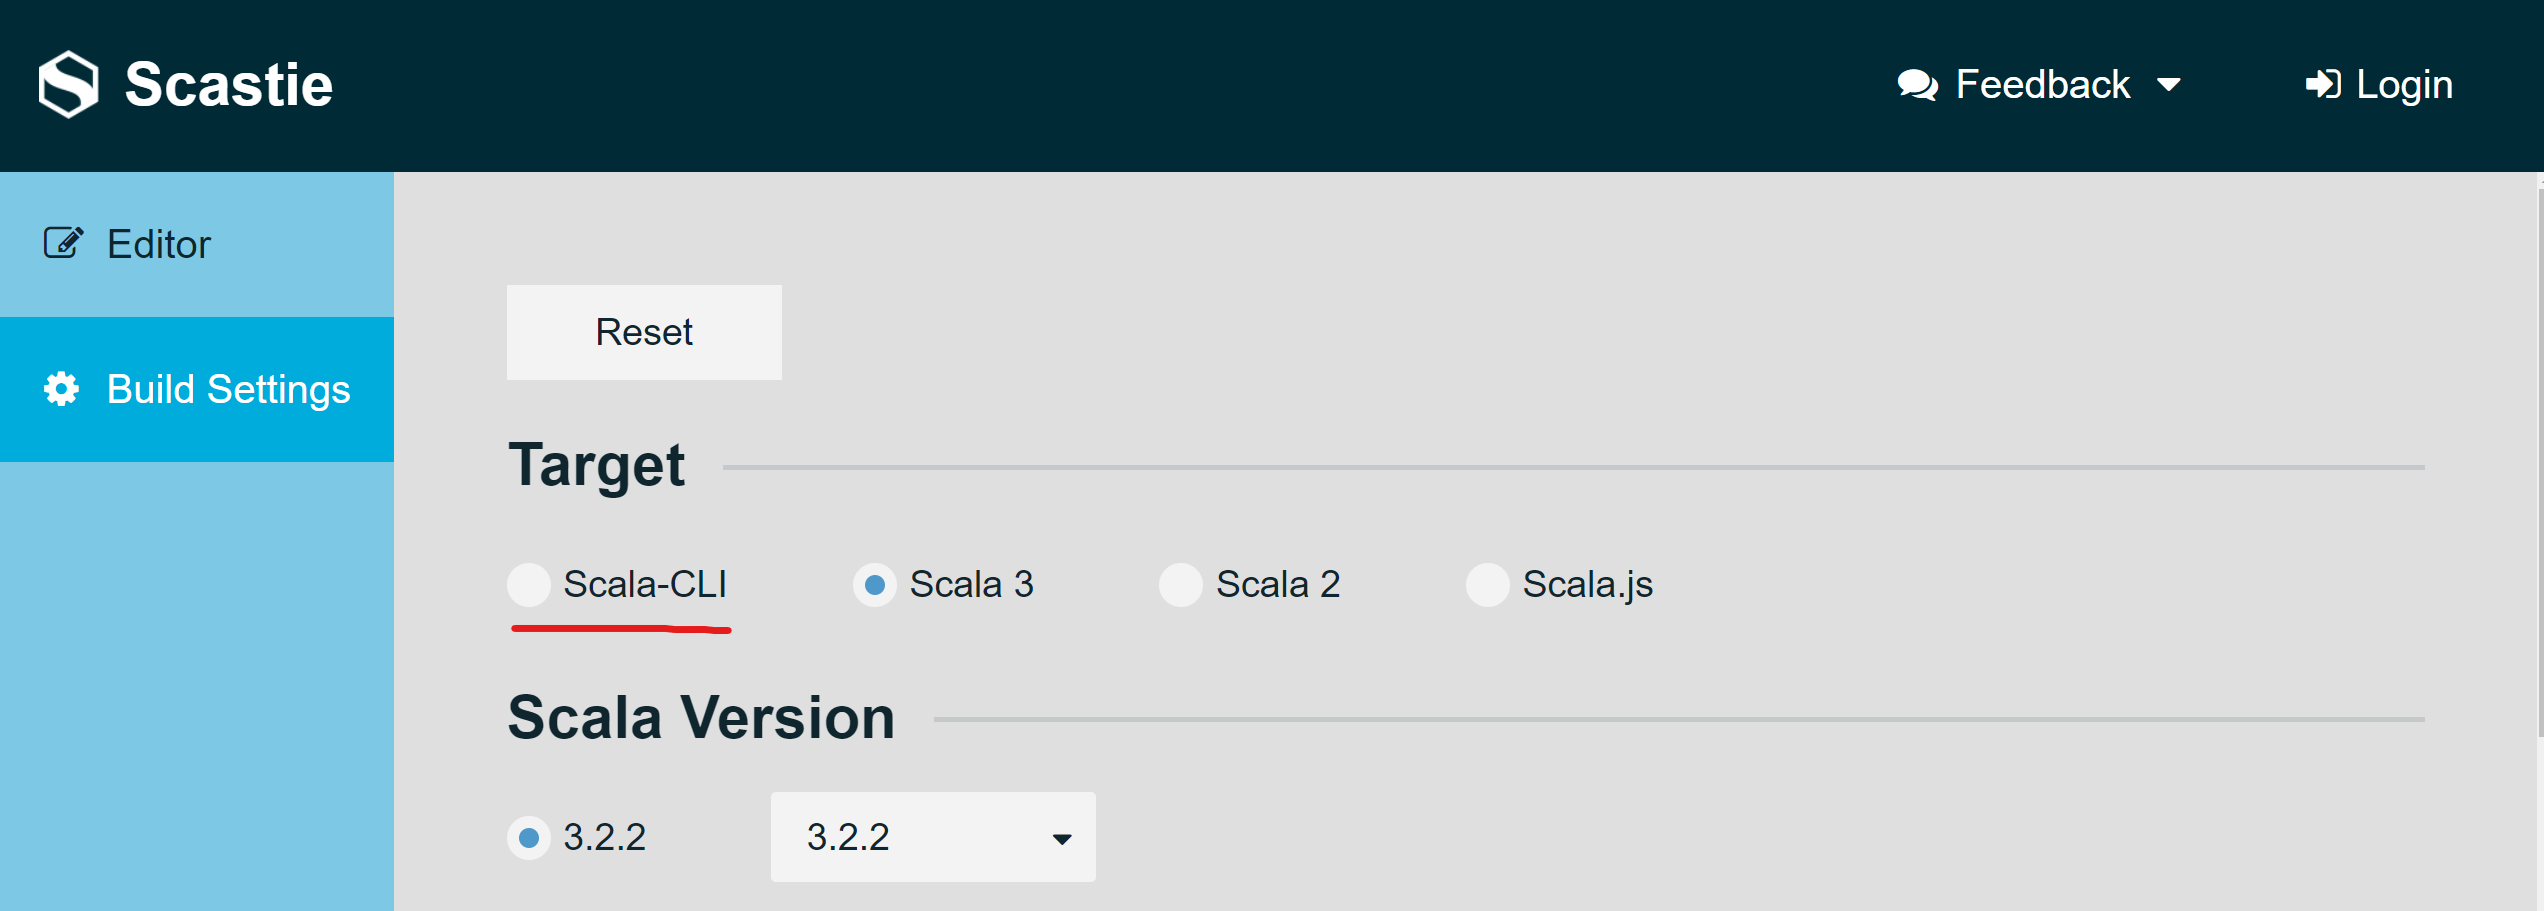
\includegraphics[width=\linewidth]{./scastie_newtarget.png}
    \caption{The new target}
\end{figure}

Since time allowed for extra work, a button has been set-up to allow the user to convert almost seamlessly (under the condition that no extra SBT configuration has been added) from SBT to Scala-CLI~:

\begin{figure}[H]
    \centering
    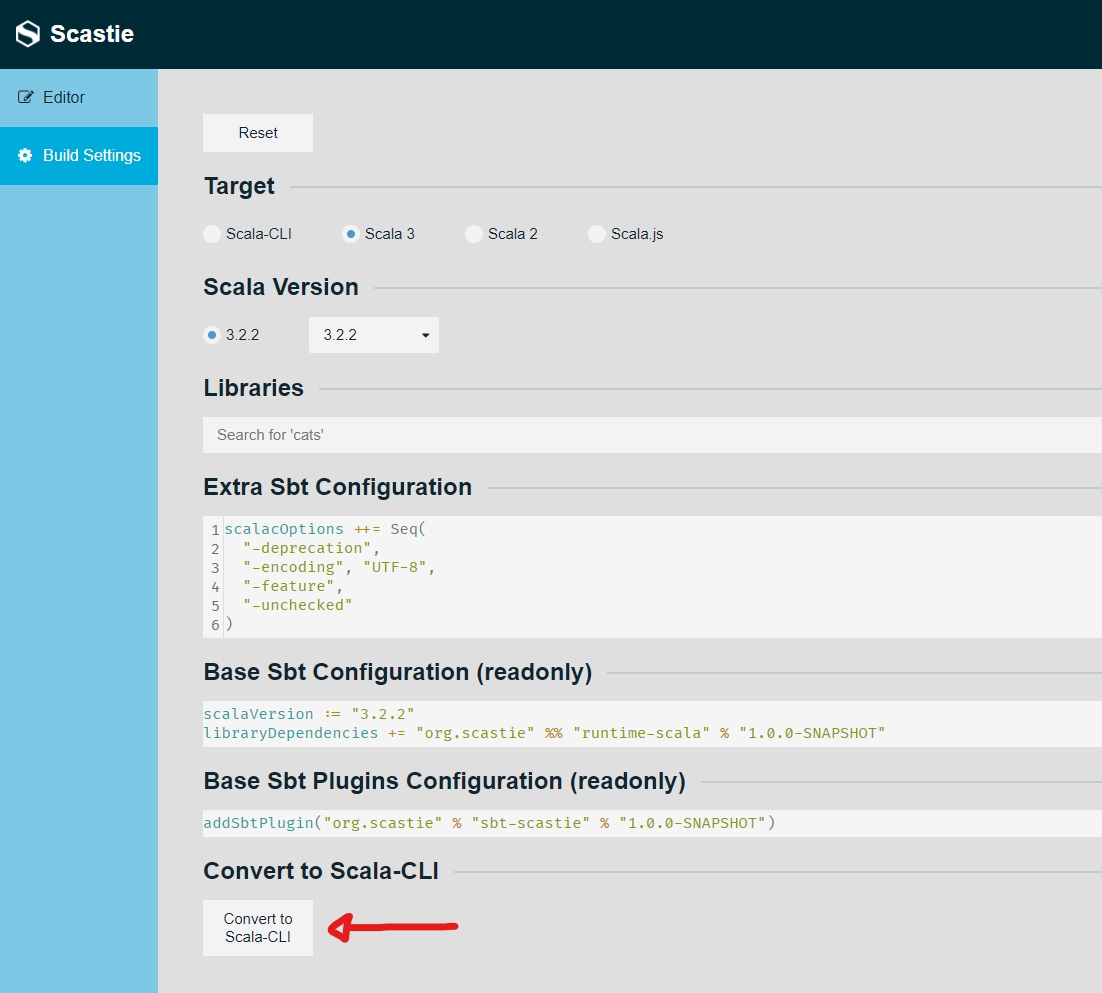
\includegraphics[width=\linewidth]{./scastie_convert.png}
    \caption{The convert button}
\end{figure}

Its behavior is not really surprising~:

\begin{itemize}
    \item Checks whether any SBT extra-configuration has been added. If yes, abort.
    \item Change the Scala target to the Scala CLI target.
    \item Prepend the code with the following~:
    \begin{itemize}
        \item \lstinline{//> using scala "<scala-version>"} with \lstinline{<scala-version>} being the Scala version of the snippet.
        \item For each dependency~: \lstinline{//> using dep "<dependency.groupId>::<dependency.artifact>::<dependency.version>"} with \lstinline{<dependency.groupId>}, \lstinline{<dependency.artifact>} and \lstinline{<dependency.artifact} being respectively the dependency's \lstinline{groupId}, \lstinline{artifact}'s name and \lstinline{version} the version.
        \item \lstinline{"========"} to separate the directives from the user code.
    \end{itemize}
\end{itemize}

\section{Metals support}

As shown in the figure \ref{fig:scastie_architecture}, the Metals server is totally independent from the Scastie server and the runners. Therefore, we need to make Metals understand the Scala-CLI directives.

Let note that the auto-completion of the \lstinline{//> using dep} is already there by default on Metals when worksheet mode is disabled. To understand why, we need to look at the Metals architecture.

\subsection{Introduction to the Metals server}

The Metals runner uses ScalaMeta's presentation compiler. Since instantiating a presentation compiler is a costly operation, Metals keeps a single instance of it and reuses it for every request~: there is no idea of a session, every request does not contain session details and the only thing that matters is the configuration of the snippet.

Here is a quick overview of how the Scastie client and the Metals server interact, hence a quick list of the endpoints that matter~:

\begin{itemize}
    \item \lstinline{/isConfigurationSupported}~: sent out by the client containing a \href{https://github.com/Maeeen/scastie/blob/main/api/src/main/scala/com.olegych.scastie.api/ApiModels.scala#LL132C101-L132C101}{\lstinline{ScastieMetalsOption(dependencies: Set[ScalaDependency], scalaTarget: ScalaTarget)}}
    
    \item \lstinline{/complete}~: sent out by the client containing a \href{https://github.com/Maeeen/scastie/blob/23e0fa998565a37d8ecfa36fa64d1268a9c1d12c/api/src/main/scala/com.olegych.scastie.api/ApiModels.scala#L169}{\lstinline{LSPRequestDTO(options: ScastieMetalsOption, offsetParams: ScastieOffsetParams)}}
    \item and other similar requests to get documentation where every of them contains a \lstinline{ScastieMetalsOption} with a \lstinline{ScastieOffsetParams} to give the cursor's position.
\end{itemize}

When a client wants to make any of these requests, it should first of all probe the Metals runner to know whether the current configuration of the user is supported ; then it can make the \lstinline{/complete} request or similar. Note that in fact the \lstinline{/isConfigurationSupported} is not mandatory, but it is a good practice to actually show to the user that the configuration is not supported.

\subsection{Worksheet mode?}

Let's recall that this auto-completion provided by ScalaMeta's presentation compiler is similar to the one that one may have in an IDE. With this supposition, the presentation compiler expects a totally valid Scala project's code.

Hence, in worksheet mode, it needs proper instrumentation. In this case, it is easier than before. It consists of only adding the following (and doing proper modifiations to the offset which is adding the indentation offset and the length of \lstinline|object worksheet {\n|)~:

\begin{lstlisting}
object worksheet {
    <user code>
}
\end{lstlisting}

With this in mind, we can understand why the \lstinline{//> using dep} was working without worksheet mode. When worksheet mode is disabled, the said instrumentation is then disabled and auto-completes as desired.

The chosen solution to split the user code as done in the Scala-CLI runner's instrumentation part.

\begin{lstlisting}
<user directives>
object worksheet {
    <user code>
}
\end{lstlisting}

When the user is making such a request, we need to appropriately take into consideration the given offset of the cursor. If the cursor is located in the directives, we do nothing. Otherwise, we need to appropriately offset it by \lstinline|object worksheet {\n|.

One may read the code that handles this on the following file \href{https://github.com/Maeeen/scastie/blob/main/metals-runner/src/main/scala/scastie/metals/DTOExtensions.scala}{metals-runner/src/\ldots/DTOExtensions.scala}

\subsection{Adding auto-completion of dependencies}

To enable such an auto-completion, dependencies should be parsed and resolved at some point. Multiple solutions have been thought~:

\begin{enumerate}
    \item Parse the directives and resolve dependencies client-side
    \item Parse the directives and resolve dependencies on the Metals runner's end
    \item Parse the directives and resolve dependencies on the Sala-CLI's runner end and make the client aware of it, then make appropriate requests to the Metals runner with these information.
\end{enumerate}

The first choice is something that costs too much to the client to do. We want it to be lightweight so that it can run on any device. Keep in mind that we have to make it "refreshable" (i.e. when adding a dependency, either client or servers should be aware of such changes and give proper auto-completions).

The last choice is too complex and involves creating new transmissions channels amongst totally independent components.

One can try to make it simple and the second solution has been chosen~: parse the directives server side, check whether all the dependencies are compatible and return a \lstinline{ScastieMetalsOption} with the Scala version and the dependencies. The client will have to send the \lstinline{ScastieMetalsOption} in every request so that every call that worked using traditional targets will work with this specific \lstinline{ScastieMetalsOption}. This will be discussed further, in the next subsection :).

%% TALK ABOUT PARSING IN THE NEXT SUBSECTION

\subsection{Adding support for directives}

With directives, users can specify the dependencies and the Scala version directly in the code. To know whether the current configuration is supported, we need to know the directives (hence the code). In this case, we need to pack the \lstinline{ScastieMetalsOption} with the code. Note that some endpoints requires a \lstinline{ScastieOffsetParams} that already contains the code. One approach of modifying the huge codebase was to make only additions and not deletions, to avoid breaking anything.

With this in mind, the endpoint \lstinline{/isConfigurationSupported} will return a \lstinline{ScastieMetalsOption}





On the runner end, VirtusLab provides a library \lstinline{using_directives} to parse these directives, available on \href{https://github.com/VirtusLab/using_directives}{Github} and \href{https://mvnrepository.com/artifact/org.virtuslab.scala-cli/directives_3}{Maven}.

\end{document}